\documentclass[t]{beamer}
\usepackage{CJKutf8}
\usepackage{amsfonts}
    \usepackage{amsmath}
    \usepackage{amssymb}
    \usepackage{amsthm}
    \usepackage{enumerate}
    \usepackage{graphicx}
    \usepackage{layout}
    \usepackage{mathrsfs}
    \usepackage{fancyhdr}
    \usepackage{subfigure}
    \usepackage{tcolorbox}
    \usepackage{tikz-cd}
    \usepackage{color}
    \usepackage{pifont}
    \usepackage{verbatim}
    \usepackage{mathtools}
    \usepackage{float}
    \usepackage{bm}
    \usetheme{AnnArbor}
% \usetheme{Antibes}
\usecolortheme{beaver}
% 表格
\usepackage{booktabs}
\usepackage{multirow}

% \setbeamertemplate{navigation symbols}{}

\usepackage{textpos}

\newcommand{\dif}{\mathrm{d}}
\newtheorem{thm}{{定理}}

% some common command
\newcommand{\mm}[1]{$ #1$\newline}
% \newcommand{\tuichu}{\Rightarrow}
% \newcommand{\li}[1]{\newline#1}



\newcommand{\analysis}[2]{\forall \mathcal{E}{#1},\exists \delta {#2},s.t.}
\newcommand{\denyanalysis}[2]{\exists \mathcal{E}{#1},\forall \delta {#2},s.t.}
\newcommand{\yield}{\Rightarrow }
\newcommand{\jj}{\newline}
\newcommand{\ff}[1]{$ #1$}   % math environment + newline
\newcommand{\fgn}[1]{\begin{equation}#1\end{equation}  }
\newcommand{\fg}[1]{$$ #1$$}   % math environment + newline 
\newcommand{\pf}{$proof.$\newline}
\newcommand{\ee}{\newline\ff{\Box}\newline}
\newcommand{\fenshi}[2]{\ff{\frac{#1}{#2}}}
\newcommand{\shenlue}{\vdots\jj}
\newcommand{\abs}[1]{{\left \lvert #1 \right\rvert}}
\newcommand{\loge}[1]{In ({#1})}
\newcommand{\logical}[2]{log_{#2}^{#1}}
\newcommand{\summary}[3]{$\sum_{{#1}={#2}}^{#3}  $}
\newcommand{\denjia}[2]{{#1}\Leftrightarrow {#2}}
\newcommand{\jihe}[3]{ {#1}  = \{ {#2} \mid {#3} \} }
\newcommand{\ve}[2]{\left\langle {#1},{#2}\right \rangle}
\newcommand{\dakuohao}[2]{\begin{array}{rcl}{#1}\end{array} \} \Rightarrow{#2}}
\newcommand{\sxb}[3]{#1^{#2}_{#3}}
\newcommand{\sss}[2]{#1^{#2}}
\newcommand{\xxx}[2]{#1_{#2}}
\newcommand{\bri}[1]{\uppercase\expandafter{\romannumeral#1}}
\newcommand{\ri}[1]{\romannumeral#1} 
\newcommand{\polynomial}[8]{#1_{#2}#6^{#7}+#1_{#3}#6^{#8}+...+#1_{#4}#6+#1_{#5} }
\newcommand{\newd}[4]{f[{#1}_{#2},{#4},{#1}_{#3}]}
\newcommand{\lb}[2]{\begin{align*}\begin{split}{#1}\{ {#2}\end{split}\end{align*}}
\newcommand{\tab}[1]{\begin{array}{ll} {#1}\end{array}}


% 向量乘积
\newcommand{\avg}[1]{\left\langle #1 \right\rangle}
% 偏微分方程
\newcommand{\difFrac}[2]{\frac{\dif #1}{\dif #2}}
\newcommand{\pdfrac}[2]{\frac{\partial{#1}}{\partial{#2}}}
% 不同章节
\newcommand{\one}[1]{\section{#1}}
\newcommand{\two}[1]{\subsection{#1}}
\newcommand{\three}[1]{\subsubsection{#1}}
\newcommand{\aone}[1]{\section*{#1}}
\newcommand{\atwo}[1]{\subsection*{#1}}
\newcommand{\athree}[1]{\subsubsection*{#1}}
% 大括号,左右都有
\newcommand{\lbra}[1]{\left\{  {\begin{matrix} #1 \end{matrix}}\right. } 
% 样式 括号前缀 + 括号 
\newcommand{\lbras}[2]{{#1}\left\{ {  {\begin{matrix} #2 \end{matrix}}}\right. } 
\newcommand{\rbra}[1]{ \left.  {\begin{matrix} #1 \end{matrix}} \right\}  } 
% 模长
\newcommand{\distance}[1]{\parallel #1\parallel }
% 等价
\newcommand{\equ}{\Longleftrightarrow }
% 共轭
\newcommand{\cja}[1]{\overline{#1}}
% 两个矩阵,上面是 方框[] 下面是线条| 中间是 无
\newcommand{\mtx}[1]{\begin{matrix}#1\end{matrix} }
\newcommand{\bmtx}[1]{\begin{bmatrix}#1\end{bmatrix} }
\newcommand{\vmtx}[1]{\begin{vmatrix}#1\end{vmatrix} }
% \newcommand{\table}[1]{\begin{array}[lr]{ccc} #1 \end{array}}

%输入普通字符
\newcommand{\ww}[1]{\text{#1}}

% 所有内容 直接头文件搞定
\newcommand{\everything}[1]{\begin{document}\begin{CJK*}{UTF8}{gkai}#1\end{CJK*}\end{document}}


% 存放代码(失败了)
\newcommand{\cccode}[1]{\begin{lstlisting}#1\end{lstlisting}}

% 改变特定行序列
\newcommand{\ttt}{\subsection{}}

% 嵌套序号
\newcommand{\eee}[1]{\begin{enumerate}#1\end{enumerate}}


% 模板里面的一些宏
\newcommand{\pdfFrac}[2]{\frac{\partial #1}{\partial #2}}
\newcommand{\OFL}{\mathrm{OFL}}
\newcommand{\UFL}{\mathrm{UFL}}
\newcommand{\fl}{\mathrm{fl}}
\newcommand{\op}{\odot}
\newcommand{\Eabs}{E_{\mathrm{abs}}}
\newcommand{\Erel}{E_{\mathrm{rel}}}
% 变化颜色
\newcommand{\red}{\textcolor{red}}
\newcommand{\blue}{\textcolor{blue}}



% 流程图需要用到的宏包
\usepackage{palatino}
\usepackage{tikz}
\usetikzlibrary{shapes.geometric, arrows}
\tikzstyle{startstop} = [rectangle, rounded corners, minimum width = 2cm, minimum height=1cm,text centered, draw = black, fill = red!40]
\tikzstyle{io} = [trapezium, trapezium left angle=70, trapezium right angle=110, minimum width=2cm, minimum height=1cm, text centered, draw=black, fill = blue!40]
\tikzstyle{process} = [rectangle, minimum width=3cm, minimum height=1cm, text centered, draw=black, fill = yellow!50]
\tikzstyle{decision} = [diamond, aspect = 3, text centered, draw=black, fill = green!30]
% 箭头形式
\tikzstyle{arrow} = [->,>=stealth]
% 4个非常重要 的新命令
\newcommand{\start}[2]{    \node (start) [startstop]{#1};\node (in1) [io, below of = start]{#2};\lin{start}{in1}{}}
\newcommand{\stopp}[3]{\node (out1) [io, below of= #1]{#2};\node (stop) [startstop, below of=out1]{#3};\lin{out1}{stop}{} }
\newcommand{\pro}[6]{    \node (#3) [process, #2 of=#1,xshift=#4 cm]{#5};}
\newpage
\newcommand{\lin}[3]{\draw [arrow] (#1) --node [above] {#3} (#2);}


\begin{document}
\begin{CJK*}{UTF8}{gkai}
% 一般第一页显示PPT标题以及作者信息

% \BackgroundPic{./Screenshot from 2022-04-20 16-31-08.png}

% 增加学校 前面
\addtobeamertemplate{title page}{}{
	\begin{tikzpicture}[remember picture,overlay]
		% \node[yshift=85pt,xshift=50pt]{\includegraphics[height=2cm]{Screenshot from 2022-04-20 16-51-21.png}};
\end{tikzpicture}
}


	\title{时间序列预测的指令微调}
	\subtitle {} %不需要
	\author{
		陈钶杰\, \\
		专业:计算数学\,
	} % 显示作者
	% \institute {学院:数学科学学院} % 设置学院机构	
	\date{\today}  % 显示日期
\titlepage

% 设置目录
\begin{frame}{目录}
\frametitle{目录}	
\tableofcontents  % 显示目录
\end{frame} 



\section{建模的基本想法}

\begin{frame}
	\frametitle{建模目标:具有一定泛化能力的时间序列预测模型}	
	\textcolor{red}{具体任务:}
    \begin{itemize}
		\item 在单个数据集中通过指令微调使得最终效果变好.
		% \eee{
		% 	\item 得到一个面向时间序列的指令微调的数据集合
		% 	\item 比较模型在增加指令以后,预测的精准度是否有提高
		% 	% \item 证明这种指令微调确实对最终的结果有用.
		% }
		\item 此模型能够接受多种指令微调的数据集合,并在这些数据集上的预测有比较好的表现.
		% \eee{
		% 	\item 还在尝试
		% }
		\item 此模型在接受一个未知的数据集也能作出相应的预测.
		% \item 语言模型,时间序列预测模型的区别:?????
		\end{itemize}
\end{frame}

\section{语言模型的指令学习}

\begin{frame}
	\frametitle{指令微调的文献-谷歌FLAN模型}
    \begin{itemize}
		\item
		\textcolor{red}{文章内容:}
		\begin{itemize}
		% \item 本文探讨了一种提高语言模型零样本学习能力的简单方法,通过指令描述的任务集合的指令调优,提高了对未知任务的零样本性能。我们采用一个137B参数的预训练语言模型,并通过自然语言指令模板对60多个NLP任务进行指令调优,在看不见的任务类型上评估这个指令调整模型.这个模型称为FLAN,即Finetuned Language Net.FLAN大大提高了未经修改的同类NLP任务的性能,并在我们评估的25个任务中的19个任务上超过了零样本175B GPT-3模型。同时,研究表明任务数量和模型规模是教学调整成功的关键组成部分。
		\item 什么是指令微调
		\item 指令微调的优点
		\item 指令微调的缺点
		\end{itemize}
	\end{itemize}
\end{frame}

\begin{frame}
	\frametitle{什么是指令微调(语言模型)}
	% \includegraphics*[scale=0.2]{png/all_prompt.png}
    \begin{itemize}
		\item fine-tuning:需要对原始数据集中每一个数据进行标记,训练.这就需要所有的数据训练库,比如情感分类,我要通过对语言库中所有的语句进行标记,这显然消耗巨大.
		\item prompting:根据单个任务给一个特定标记的数据集,用这个特定标记的数据集来训练模型,其中这个标记的数据集规模可能远小于语言库中的数据集.促使模型能够完成此任务.
		\item instruction tuning 是通过在多个任务上添加提示,得到指令微调的数据集进行微调模型,能在一个未见过的任务上有良好的表现.
		\end{itemize}
\end{frame}


\begin{frame}
	\frametitle{指令微调的优点}
    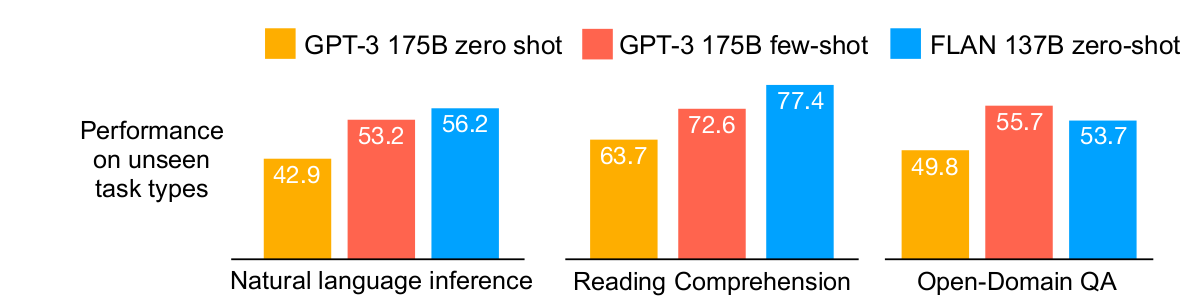
\includegraphics[scale=0.27]{png/gpt_3_flan.png}\\
		1.对于未见过的任务,FLAN模型的效果最好,甚至超越比他参数更多的gpt-3模型.
\end{frame}




\begin{frame}
	\frametitle{指令微调的优点}

		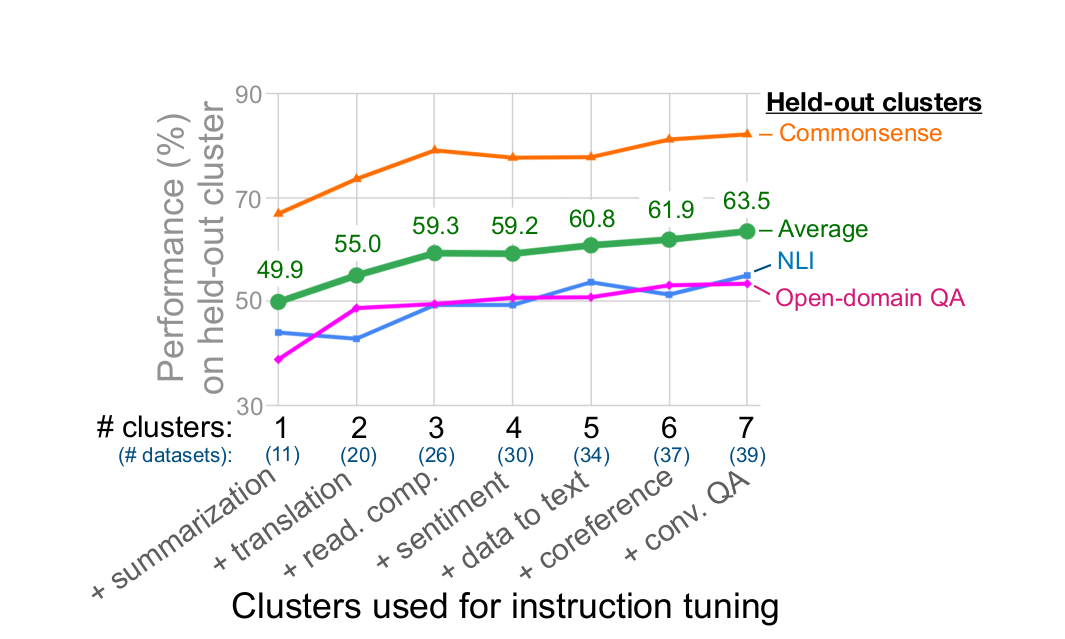
\includegraphics[scale=0.25]{png/much_task.png}\\
		2.从图表中可以看出,当指令微调的任务越多,最终模型在完成没见过的任务上表现越好.

\end{frame}

\begin{frame}
	\frametitle{指令微调的优点}
		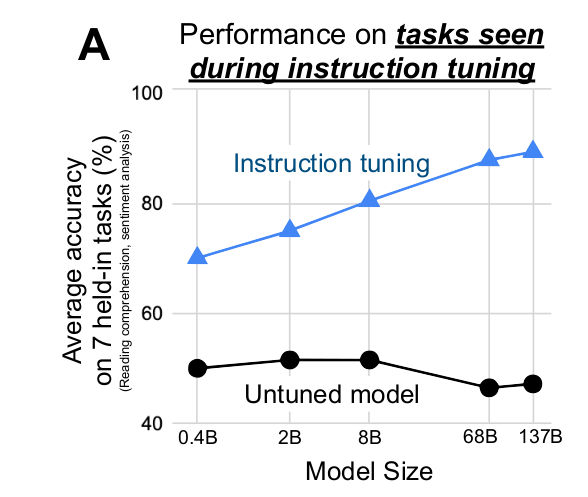
\includegraphics[scale=0.3]{png/use_instruction.png}\\
		3.从图表中可以看出,在可见的任务上,使用指令微调的效果比不使用要好很多.而且随着数据数据的变多效果会更加好.
\end{frame}




\begin{frame}
	\frametitle{指令微调的缺点}
	
		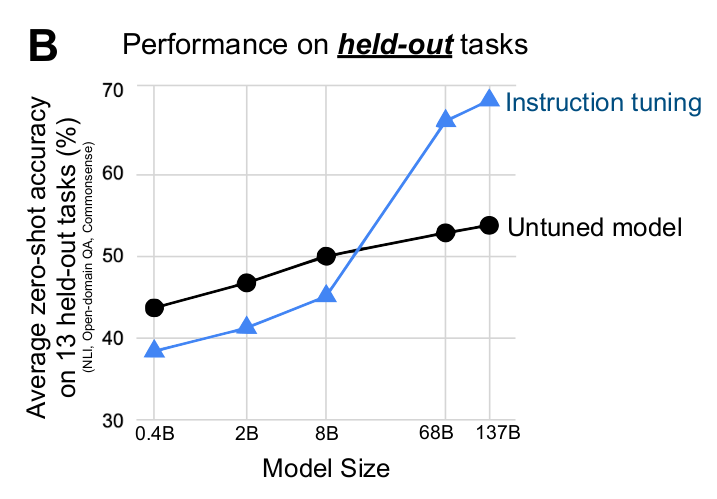
\includegraphics[scale=0.23]{png/bad_instruction.png}\\
1.从图中可以知道,在完成未知任务的时候,只有在模型参数超过10B的时候,FLAN模型才才比不微调的模型效果好

		原因:可能是在训练过程中,这个指令微调用掉了许多的参数.如果参数不够多的,指令微调就会用掉大量的参数,导致最终模型过拟合,在其他数据集上的效果反而变得更差.
\end{frame}

\begin{frame}
	\frametitle{指令微调的缺点}
	2. 不同任务的表现不一样
			\begin{itemize}
				\item 在一些任务上很有用:translation(翻译)
				\item 在一些任务上没啥用:coreference roslolution(指代消解)
			\end{itemize}
			在这里指代消解就是将代词替换成具体指代的内容,这个就像是完形填空,和预处理的任务很相似,所以增加instructions反而显得冗余.
	\end{frame}
\section{时间序列预测的指令微调}

\begin{frame}
	\frametitle{对时间数据进行}
	\textcolor{red}{模型选择}
	\begin{itemize}
		\item 使用的函数序列测试,故使用的时间预测模型是DLinear,使得效果更好,速度更快.
		\item 测试序列的总长度是30000,21000个数据用作训练,3000个数据用作验证,6000数据用作测试,数据是按顺序选取.
		\item 
		\eee{
			\item seq\_len:60
			\item pred\_len:10
		}
	\end{itemize}
\end{frame}

\begin{frame}
	\frametitle{面向时间序列的指令微调的数据集}
    \begin{itemize}
		\item 
		\textcolor{red}{构建常用函数的一个时间序列}
		\begin{itemize}
		\item 构建了一个如下的函数时间序列:\\
		\ff{
			\mtx{
			f1:x 	& f2:sin(x^2+2)& f3:\cos(x) & f4:\sin(x)  \\
			1 		& sin(1^2+2) &\cos(1)  & \sin(1) \\
			\vdots  &\vdots 	 &\vdots   & \vdots\\
			n  		&\sin(n^2+2) &\cos(n)  & \sin(n) \\
			\vdots  &\vdots 	 &\vdots   & \vdots\\
			}	
		}
		\item 对于一个时间序列,我们一般关注其中某个维度的信息,我们这边更关注sin(x)即第四个维度上的预测,模型最终的mse,mae是计算第四个维度的预测误差.
		\end{itemize}
		\item 计算结果:
		\fg{
			\mtx{
				MSE:0.2742\\
				MAE:0.2513
			}
		}
	\end{itemize}
\end{frame}



\begin{frame}
	\frametitle{面向时间序列的指令微调的数据集}
    \begin{itemize}	
		\item 
		\textcolor{red}{添加合适的指令微调}
		\begin{itemize}
		\item \ff{\sin(x)}是一种周期函数,所以简单想法就是增加一个周期性函数,来起到对这个提示的效果:
		\item 构建了一个如下的微调的函数时间序列:\\
		\ff{
			\mtx{
			f1:x 	& f2:sin(x^2+2)& f3:\cos(x) & f4:\sin(x) & f5: x \% 4\\
			1 		& sin(1^2+2) &\cos(1)  & \sin(1) & 1 \% 4\\
			\vdots  &\vdots 	 &\vdots   & \vdots  & \vdots \\
			n  		&\sin(n^2+2) &\cos(n)  & \sin(n) & n \% 4 \\
			\vdots  &\vdots 	 &\vdots   & \vdots  & \vdots \\
			}	
		}
		\end{itemize}
		\item 最终计算结果\\
		\fg{
			\mtx{
				MSE:0.2321\\
				MAE:0.2112
			}
		}
	\end{itemize}
\end{frame}


\begin{frame}
	\frametitle{面向时间序列的指令微调的数据集}
    \begin{itemize}	
		\item 
		\textcolor{red}{错误的提示会带来更大的误差}
		\begin{itemize}
		\item 把提示改成一个非周期的函数f5:\ff{\frac{(sin(x^2+2)+cos(x)+sin(x))}{3}}
		\item 构建了一个如下的微调的函数时间序列:\\
		\ff{
			\mtx{
			f1:x 	& f2:sin(x^2+2)& f3:\cos(x) & f4:\sin(x) & f5: \frac{sin(x^2+2)+cos+sin}{3}\\
			\vdots  &\vdots 	 &\vdots   & \vdots  & \vdots \\
			}	
		}
		\end{itemize}
		\item 最终计算结果\\
		\fg{
			\mtx{
				MSE:0.2935\\
				MAE:0.3110
			}
		}
	\end{itemize}
\end{frame}

\begin{frame}
	\frametitle{}
    \begin{itemize}	
		\item 
		\textcolor{red}{对于未知特征的序列如何提示}
		\begin{itemize}
		\item sin(x)我们是知道他有周期性的,但是实际的序列的性质我们是未知的,这个时候要如何通过提示?\\
		序列自己本身就是一种很好的提示!
		\item 构建了一个如下的微调的函数时间序列:\\
		\ff{
			\mtx{
			f1:x 	& f2:sin(x^2+2)& f3:\cos(x) & f4:\sin(x) & f5:\sin(x)\\
			\vdots  &\vdots 	 &\vdots   & \vdots  & \vdots \\
			}	
		}
		\end{itemize}
		\item 最终计算结果\\
		\fg{
			\mtx{
				MSE:0.2214\\
				MAE:0.2016\\
			}
		}
	\end{itemize}
\end{frame}

\begin{frame}
	\frametitle{}
    \begin{itemize}	
		\item 
		\textcolor{red}{对于未知特征的序列如何提示}
		\begin{itemize}
		\item 还可以考虑删除序列中相关性比弱的序列,比如这边删除那个相关性比较弱的序列\ff{sin(x^2+2)}
		\item 构建了一个如下的微调的函数时间序列:\\
		\ff{
			\mtx{
			f1:x 	& f3:\cos(x) & f4:\sin(x)\\
			\vdots  &\vdots   & \vdots  \\
			}	
		}
		\end{itemize}
		\item 最终计算结果\\
		\fg{
			\mtx{
				MSE:4.566e-06\\
				MAE:0.00201
			}
		}
	\end{itemize}
\end{frame}

\begin{frame}
	\frametitle{}
    \begin{itemize}	
		\item 
		\textcolor{red}{总结}
		\begin{itemize}
		\item 可以通过增加一列目标值相同的序列,比如上面的\ff{sin(x)}来对数据起到微调作用.
		\item 通过计算一个向量各个维度的序列之间的相关系数来考虑删减某一列.
		\end{itemize}
		\item \textcolor{red}{下一步计划}
		\begin{itemize}
			\item 思考如何在同一个模型里面,尝试使用指令微调对多种不同的数据集进行训练,能够使得模型能够在已知数据集上通过微调后有更好的表现.
		\end{itemize}		
	\end{itemize}
\end{frame}

\begin{frame}
	\frametitle{}
    \begin{itemize}	
		\item \textcolor{red}{问题}
		\begin{enumerate}
			\item 对于多种不同数据集合,最终对于每种序列的预测维度都是指定的吗?
			\item 时间序列和自然语言处理模型之间是有显著差异的.
			
			比如对于语言模型而言,
			\begin{itemize}
				\item 情感分类问题的提示可以是:这部电影很有趣,这个电影是[好看的]
				\item 翻译任务的提示可以是:这部电影很有趣,这个电影的英文表示是[movie]
				\item 去解决没有遇到过的问题比如是代词指代:这部电影很有趣,它的剧情很好,这个它的指代是[这部电影]
			\end{itemize}
			未见的任务,还是和已有的任务有一定的关联性的,但对于两个不同的时间序列而言,两者之间是完全没有关系的,比如:
			\begin{itemize}
				\item 一个是任务是预测序列 log(x)
				\item 			另一个是任务是预测序列 \ff{\sqrt{x}}
				\item 			未见的任务是预测序列 sin(x)
			\end{itemize}
			未见序列sin(x)和前面 已有的两个序列都没关系.

			所以可能对最终预测数据集合是有一定要求的.
		\end{enumerate}

	\end{itemize}
\end{frame}



\section{}
\begin{frame}
	\frametitle{}
	\begin{center}
		\Huge{谢谢老师和同学的聆听!}
	\end{center}
\end{frame}


\end{CJK*}
\end{document}